
\documentclass{article}
\usepackage[final]{neurips_2019}

\makeatletter
\renewcommand{\@noticestring}{Deep Learning, Sommer 2019, Universiteit van Amsterdam}
\makeatother

\usepackage{comment}
\usepackage{amsmath}
\usepackage{amssymb}
\usepackage{multirow}
\usepackage{verbatim}

\usepackage{hyperref}
\usepackage{algorithm}
\usepackage{algpseudocode}
\usepackage{nicefrac}
\usepackage{graphicx}
\usepackage{caption}
\usepackage{subcaption}
\usepackage{dsfont}
\usepackage{bm}
\usepackage[utf8]{inputenc}
\usepackage[T1]{fontenc}
\usepackage{url}
\usepackage{booktabs}
\usepackage{microtype}
\usepackage{tabularx}

% Matrices
\newcommand\bM[1]{\ensuremath{\begin{bmatrix}#1\end{bmatrix}}}
\newcommand\vM[1]{\ensuremath{\begin{vmatrix}#1\end{vmatrix}}}
\newcommand\BM[1]{\ensuremath{\begin{Bmatrix}#1\end{Bmatrix}}}

% operators and fractions
\newcommand\·{\ensuremath{\cdot}}
\newcommand\…{\ensuremath{\dots}}
\newcommand\p{\ensuremath{\partial}}
\renewcommand\t{\ensuremath{\times}}
\DeclareMathOperator*{\argmax}{arg\,max}
\DeclareMathOperator*{\argmin}{arg\,min}
\DeclareMathOperator{\adj}{Adj}
\DeclareMathOperator{\Tr}{Tr}
\DeclareMathOperator{\Dir}{Dir}
\DeclareMathOperator{\sgn}{sgn}
\DeclareMathOperator{\soft}{softmax}
\DeclareMathOperator{\diag}{diag}

% unicode to latex
\newcommand{\⇔}{\ensuremath{\Leftrightarrow}}
\newcommand{\⇐}{\ensuremath{\Rightarrow}}
\newcommand{\⇒}{\ensuremath{\Leftarrow}}

\newcommand\f[2]{\ensuremath{\frac{#1}{#2}}}
\newcommand\nf[2]{\ensuremath{\nicefrac{#1}{#2}}}
\newcommand\pf[2]{\ensuremath{\frac{\partial {#1}}{\partial {#2}}}}

% Typesetting and symbols
\newcommand*{\B}[1]{\ifmmode\bm{#1}\else\textbf{#1}\fi}
\newcommand*{\I}[1]{\ifmmode\mathit{#1}\else\textit{#1}\fi}
\newcommand\1{\ensuremath{\mathds{1}}}
\newcommand\E{\ensuremath{\mathds{E}}}
\newcommand\ℝ{\ensuremath{\mathds{R}}}
\newcommand\N{\ensuremath{\mathcal{N}}}


\renewcommand{\thesubsubsection}{\thesubsection.\alph{subsubsection})}

\title{Assignment 1. MLPs, CNNs and Backpropagation}
\author{%
  Maurice Frank\\
  11650656\\
  \href{mailto:maurice.frank@posteo.de}{maurice.frank@posteo.de} \\
  Code: \href{https://github.com/morris-frank/uvadlc_practicals_2019/tree/master/assignment_1/code}{github}
}

\begin{document}
\maketitle
\section{MLP backpropagation}
\subsection{Analytical derivation of gradients}
\subsubsection{}
\begin{align*}
  \tag{$\pf{\B{x}^{(N)}}{L}$}
  \pf{L}{x_i^{(N)}}
  &= -\pf{}{x_i^{(N)}}\sum_i t_i \log x_i^{(N)}\\
  &= -t_i\·\f{1}{x_i^{(N)}}\\
  &\⇔\\
  \pf{L}{\B{x}^{(N)}}
  &= -[\dotsb \f{t_i}{x_i^{(N)}}\dotsb]\\
  &= \B{t}\oslash\B{x}^{(N)}\\
  &\in\ℝ^{d_N}
\end{align*}

\begin{align*}
  \tag{$\pf{\B{x}^{(N)}}{\tilde{\B{x}}^{(N)}}$}
  \pf{x_i^{(N)}}{\tilde{x_j}^{(N)}}
  &= \pf{}{\tilde{x}_j^{(N)}}\f{\exp{\tilde{x}_i^{(N)}}}{\sum_k \exp{\tilde{\B{x}}_k^{(N)}}}\\
  &= \f{\left(\pf{}{\tilde{x}^{(N)}_j}\exp{\tilde{x}^{(N)}_i}\right)\·\sum_k\exp{\tilde{x}^{(N)}_k} - \exp{\tilde{x}^{(N)}_i}\·\pf{}{\tilde{x}^{(N)}_j}\sum_k\exp{\tilde{x}^{(N)}_k}}{\left(\sum_k\exp{\tilde{x}^{(N)}_k}\right)^2}\\
  &= \f{\delta_{ij}\exp{\tilde{x}^{(N)}_j}}{\sum_k\exp{\tilde{x}^{(N)}_k}} - \f{\exp{\tilde{x}^{(N)}_i}\·\exp{\tilde{x}^{(N)}_j}}{\left(\sum_k\exp{\tilde{x}^{(N)}_k}\right)^2}\\
  &= \soft(\tilde{x}^{(N)}_j)\·(\delta_{ij} - \soft(\tilde{x}^{(N)}_i))\\
  &\Rightarrow\\
  \pf{\B{x}^{(N)}}{\tilde{\B{x}}^{(N)}} &= \bM{& \vdots &\\\hdots & \soft(\tilde{x}^{(N)}_j)\·(\delta_{ij} - \soft(\tilde{x}^{(N)}_i)) & \hdots\\ & \vdots &}\\
  &= \diag(\soft(\tilde{\B{x}}^{(N)})) -\soft(\tilde{\B{x}}^{(N)})\otimes \soft(\tilde{\B{x}}^{(N)})
  &\in\ℝ^{d_N\t d_N}
\end{align*}

\begin{align*}
  \tag{$\pf{\B{x}^{(l<N)}}{\tilde{\B{x}}^{(l<N)}}$}
  \pf{\B{x}^{(l<N)}}{\tilde{\B{x}}^{(l<N)}}
  &= \pf{}{\tilde{\B{x}}^{(l<N)}}\max(0,\tilde{\B{x}}^{(l<N)})\\
  &= \diag(\B{x}^{(l<N)}\oslash\tilde{\B{x}}^{(l<N)})\\
  &\in\ℝ^{d_l\t d_l}
\end{align*}

\begin{align*}
  \tag{$\pf{\tilde{\B{x}}^{(l)}}{\B{x}^{(l-1)}}$}
  \pf{\tilde{\B{x}}^{(l)}}{\B{x}^{(l-1)}}
  &= \pf{}{\B{x}^{(l-1)}} \B{W}^{(l)}\B{x}^{(l-1)} + \B{b}^{(l)}\\
  &=\B{W}^{(l)}\\
  &\in\ℝ^{d_l\t d_{l-1}}
\end{align*}

\begin{align*}
  \tag{$\pf{\tilde{\B{x}}^{(l)}}{\B{W}^{(l)}}$}
  \pf{\tilde{\B{x}}^{(l)}}{\B{W}^{(l)}}
  &= \pf{}{\B{W}^{(l)}}\B{W}^{(l)}\B{x}^{(l-1)}\\
  &= \bM{\vdots\\\pf{\tilde{\B{x}}^{(l)}_i}{\B{W}^{(l)}}\\\vdots}\\
  &\in\ℝ^{d_l\t (d_l\t d_{l-1})}\\
  &\text{with}\\
  \pf{\tilde{\B{x}}^{(l)}_i}{\B{W}^{(l)}}
  &= \bM{\vdots\\{\B{x}^{(l-1)}}^T\\\vdots}\\
  &\in\ℝ^{d_l\t d_{l-1}}
\end{align*}

\begin{align*}
  \tag{$\pf{\tilde{\B{x}}^{(l)}}{\B{b}^(l)}$}
  \pf{\tilde{\B{x}}^{(l)}}{\B{b}^{(l)}}
  &= \pf{}{\B{b}^{(l)}}\B{b}^{(l)}\\
  &= \1^{d_l\t d_l}\\
  &\in\ℝ^{d_l\t d_l}
\end{align*}

Note the use of $\oslash$ for element-wise division, the use of $\delta$ for the Kronecker-Delta and the use of $\otimes$ for the Outer Product.

\subsubsection{}
\begin{align*}
  \tag{$\pf{L}{\tilde{\B{x}}^{(N)}}$}
  \pf{L}{\tilde{\B{x}}^{(N)}}
  &= \pf{L}{\B{x}^{(N)}}\pf{\B{x}^{(N)}}{\tilde{\B{x}}^{(N)}}\\
  &= \pf{L}{\B{x}^{(N)}}\·\bM{& \vdots &\\\hdots & \text{softmax}(\tilde{x}^{(N)}_j)\·(\delta_{ij} - \text{softmax}(\tilde{x}^{(N)}_i)) & \hdots\\ & \vdots &}
\end{align*}

\begin{align*}
  \tag{$\pf{L}{\tilde{\B{x}}^{(l<N)}}$}
  \pf{L}{\tilde{\B{x}}^{(l<N)}}
  &= \pf{L}{\tilde{\B{x}}^{(l)}}\pf{\B{x}^{(l)}}{\tilde{\B{x}}^{(l)}}\\
  &= \pf{L}{\tilde{\B{x}}^{(l)}}\·\B{x}^{(l)}\oslash\tilde{\B{x}}^{(l)}
\end{align*}

\begin{align*}
  \tag{$\pf{L}{\B{x}^{(l<N)}}$}
  \pf{L}{\B{x}^{(l<N)}}
  &= \pf{L}{\tilde{\B{x}}^{(l+1)}}\pf{\tilde{\B{x}}^{(l+1)}}{\B{x}^{(l)}}\\
  &= \pf{L}{\tilde{\B{x}}^{(l+1)}}\·\B{W}^{(l+1)}\\
\end{align*}

\begin{align*}
  \tag{$\pf{L}{\B{W}^{(l)}}$}
  \pf{L}{\B{W}^{(l)}}
  &= \pf{L}{\tilde{\B{x}}^{(l)}}\pf{\tilde{\B{x}}^{(l)}}{\B{W}^{(l)}}\\
\end{align*}

\begin{align*}
  \tag{$\pf{L}{\B{b}^{(l)}}$}
  \pf{L}{\B{b}^{(l)}}
  &= \pf{L}{\tilde{\B{x}}^{(l)}}\pf{\tilde{\B{x}}^{(l)}}{\B{b}^{(l)}}
\end{align*}

\subsubsection{}
If we use batchsize\…\…\…

\subsection{NumPy MLP}
The performance of the NumPy implementation of the MLP under differnt hyperparameter settings are show in Tabel~\ref{tab:numpy}.
The loss and accuracy curves of the best model are shown in Figure~\ref{fig:numpy}.
Source code is in files \texttt{mlp\_numpy.py}, \texttt{train\_mlp\_numpy.py} and \texttt{modules.py}.

\begin{table}
  \centering
  \begin{tabular}{ccccc}
    Layers & LR & Batch size & Test Accuracy & Test Loss\\\toprule
    100 & 2e-3 & 200 & 46.86 & 1.51\\
    10 & 2e-3 & 200 & 39.38 & 1.68\\
    200 & 1e-3 & 200 & \textbf{50.37} & \textbf{1.42}\\
    80,50 & 1e-5 & 200 & 11.17 & 2.30\\
  \end{tabular}
  \caption{Results for the NumPy MLP under different parameter settings. Layers shows the sorted list of number of neurons for the hidden layers. LR is learning rate. Reported are the highest accuracy and lowest loss on the test set during training.}
  \label{tab:numpy}
\end{table}

\begin{figure}
  \begin{tabularx}{\linewidth}{XX}
    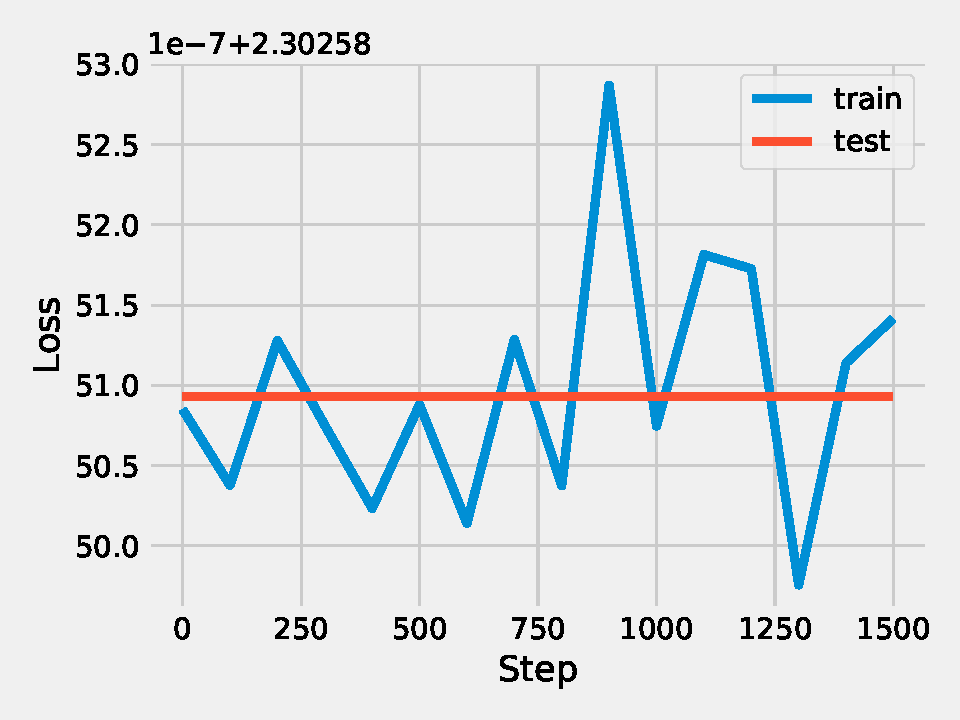
\includegraphics[width=\linewidth]{assignment_1/code/np_loss.pdf} &
    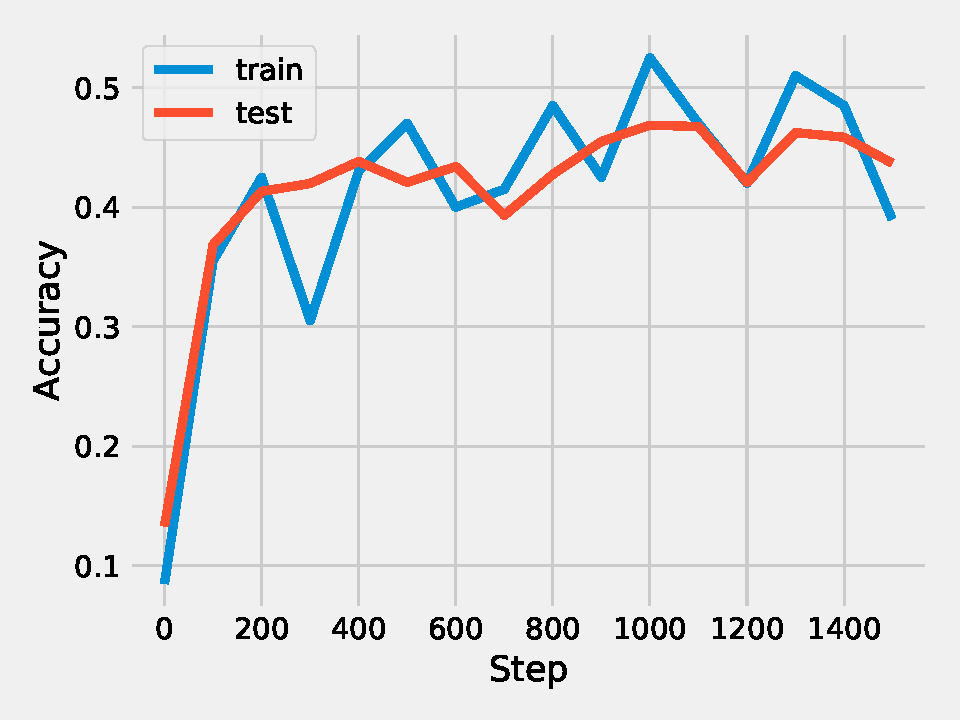
\includegraphics[width=\linewidth]{assignment_1/code/np_accuracy.pdf}
  \end{tabularx}
  \caption{\textbf{Left} the loss and \textbf{right} the accuracy during training of the NumPy MLP implementation.}
  \label{fig:numpy}
\end{figure}

\section{PyTorch MLP}
The performance of the PyTorch MLP model under diffent settings are shown in Table~\ref{tab:pytorch_mlp}.
The loss and accuracy curves during training of the best performing model are shown in Figure~\ref{fig:pytorch_mlp}.
Source code is in files \texttt{mlp\_pytorch.py} and \texttt{train\_mlp\_pytorch.py}.

\begin{table}
  \centering
  \begin{tabular}{ccccc}
    Layers & LR & Batch size & Test Accuracy & Test Loss\\\toprule
    100 & 2e-3 & 200 & 45.58 & 1.61\\
    10 & 2e-3 & 200 & 39.52 & 1.70\\
    200 & 1e-3 & 200 & \textbf{48.14} & \textbf{1.53}\\
    80,50 & 1e-5 & 200 & 31.08 & 2.26\\
    300 & 1e-5 & 200 & 33.27 & 4.25\\
  \end{tabular}
  \caption{Results of the PyTorch MLP using differnt settings for the hyperparameters.}
  \label{tab:pytorch_mlp}
\end{table}

\begin{figure}
  \begin{tabularx}{\linewidth}{XX}
    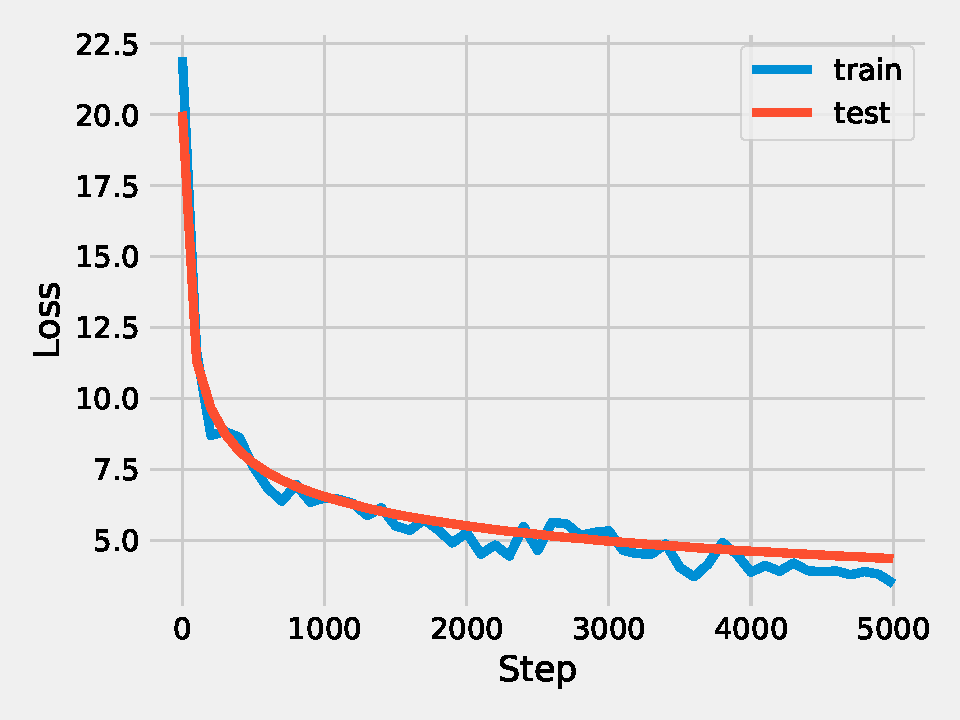
\includegraphics[width=\linewidth]{assignment_1/code/torch_loss.pdf} &
    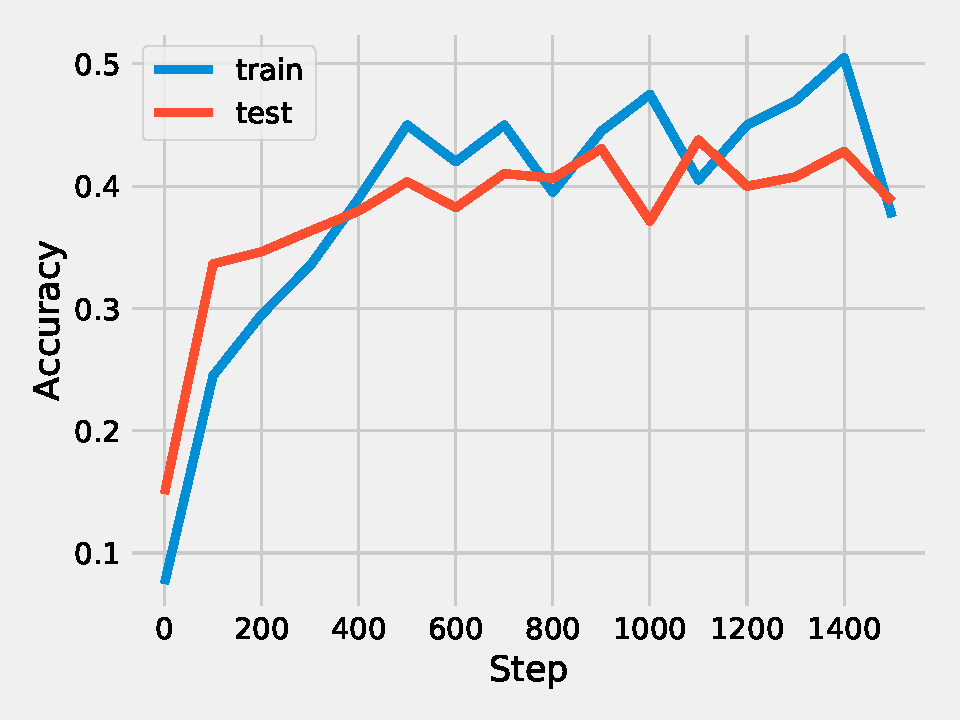
\includegraphics[width=\linewidth]{assignment_1/code/torch_accuracy.pdf}
  \end{tabularx}
  \caption{\textbf{Left} the loss and \textbf{right} the accuracy during training of the PyTorch MLP implementation.}
  \label{fig:pytorch_mlp}
\end{figure}

\end{document}
